The goal was to maintain the position of a 1kg mass hanging on a linear spring and attached to a 10kg pendulum.
The mass is actuated by vertical force and the pendulum is passive (2-DoF).
The spring is modelled by an external force of the following form:

\[
\begin{aligned}
F_{ext} = -k*Mass\_position
\end{aligned}
\addtag
\label{eq:f_ext}
\]
where k is the spring stiffness constant.


 
The first term of the objective function (Eq.~\ref{eq:ocp_Pendulum}) corresponds to the tracking of the mass position.
The second and third were added for control regularization.
The objective functions, composed of Lagrange terms, was formulated as follow:


\[\label{eq:ocp_Pendulum}
\mathcal{J} = \underbrace{\int_{T/2}^T (q_{mass} + 0.5)^2~dt}_{TRACK\_STATE}  +~\omega_1 \underbrace{\int_{T/2}^T ~\tau^2~dt}_{MINIMIZE\_ TORQUE},
\]
\noindent with $q_{mass}$ the position of the mass, $\omega_1 = 1\times 10^{-6}$, T the duration of the movement and $\tau$ the force control of the mass.


The movement was unactuated for 5 seconds, then actuated for a supplementary 5 seconds and each phase was discretized using 51 shooting nodes.
The mass actuation is able to compensate actively the spring force during the second phase of the movement stabilizing the mass around the targeted position.


\begin{figure*}[t!]
\centering
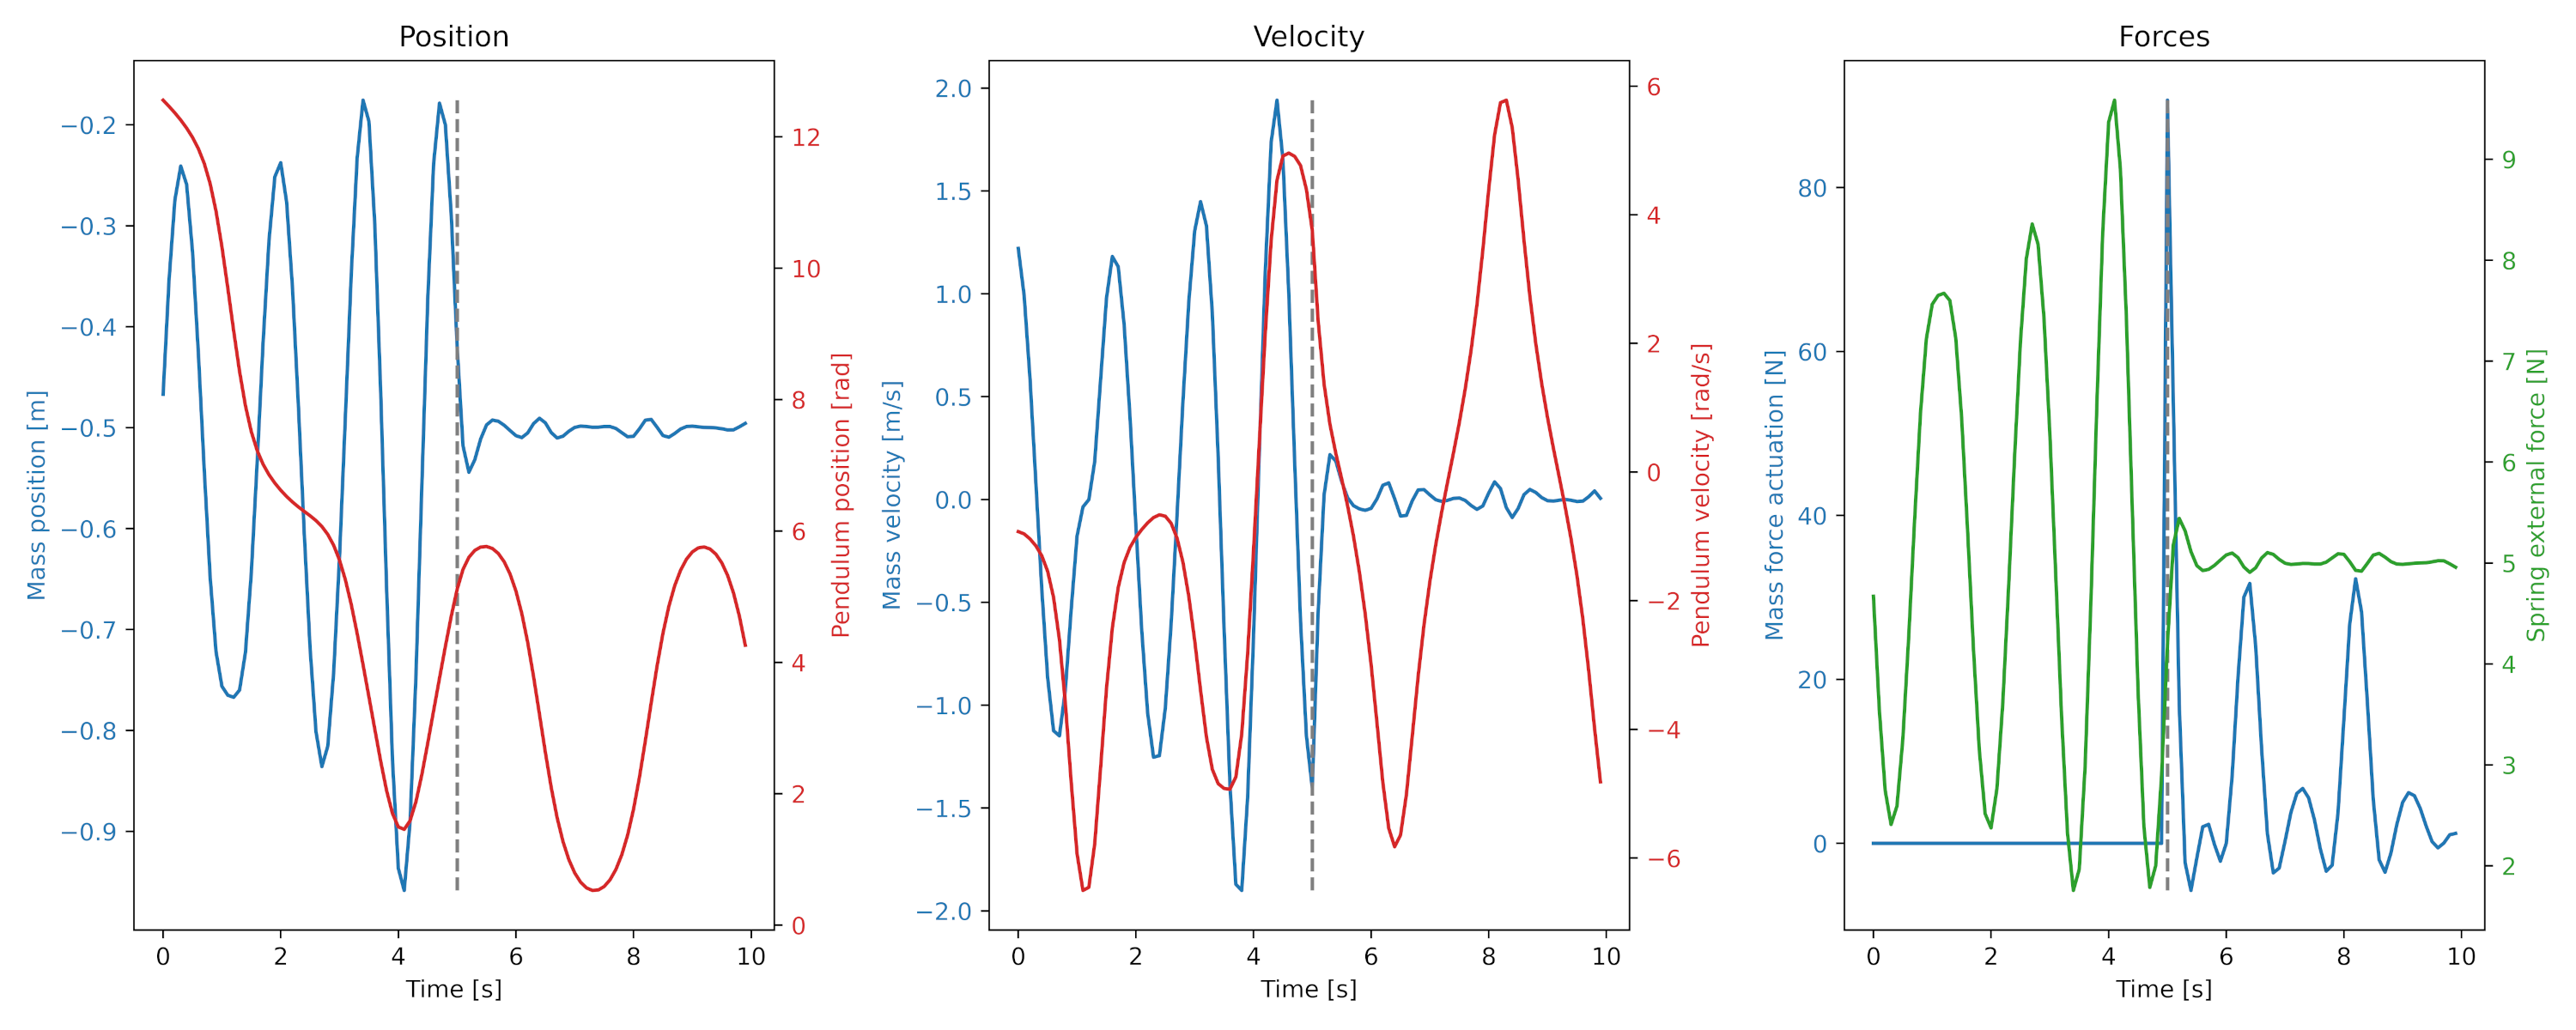
\includegraphics[width=\textwidth]{figures/Mass_Pendulum_Fext.png}
\caption{Optimal kinematics of the mass-pendulum-spring system. Gray dashed lines show the stage transition, blue lines are associated with the mass, red lines are associated with the pendulum and the green line is associated with the spring.}
\label{fig:Mass_Pendulum_Fext_graphs}
\end{figure*}














